\begin{frame}
    \frametitle{Aufgabe 9.1 - AVL Bebaumung}
    Gegeben sei ein AVL-Baum der nur aus einem Knoten mit Schlüssel 10 besteht.

    \medskip
    Fügen Sie nacheinander die Schlüssel $5, 17, 3, 1, 4$ ein.

    \smallskip
    Löschen Sie dann den Schlüssel $4$.

    \smallskip
    Fügen Sie dann die Schlüssel $8, 2, 7, 6, 9$ ein.

    \smallskip
    Löschen Sie dann die Knoten mit den Schlüsseln $2, 1, 8$.

    \medskip
    Zeichnen Sie den AVL-Baum für jede Einfüge- bzw. Löschoperation und geben Sie an,
    ob Sie keine, eine Einfach- oder eine Doppelrotation durchgeführt haben.
\end{frame}

\begin{frame}[t]
    \frametitle{Aufgabe 9.1 - AVL Bebaumung}
    Insert 5:

    \bigskip
    \bigskip

    \begin{columns}
        \begin{column}{0.48\textwidth}
            \begin{center}
                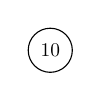
\begin{tikzpicture}[nodeStyle/.style={circle, draw, minimum size=0.8cm}, scale=0.7, transform shape]
                    \node[nodeStyle] (root) at (0, 0) {10};
                \end{tikzpicture}
            \end{center}
        \end{column}
        \begin{column}{0.48\textwidth}
        \end{column}
    \end{columns}
\end{frame}

\begin{frame}[t]
    \frametitle{Aufgabe 9.1 - AVL Bebaumung}
    Insert 17:

    \bigskip
    \bigskip

    \begin{columns}
        \begin{column}{0.48\textwidth}
            \begin{center}
                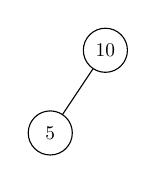
\begin{tikzpicture}[nodeStyle/.style={circle, draw, minimum size=0.8cm}, scale=0.7, transform shape]
                    \node[nodeStyle] (root) at (0, 0) {10};
                    \node[nodeStyle] (11) at (-1, -1.5) {5};

                    \draw (root) -- (11);
                \end{tikzpicture}
            \end{center}
        \end{column}
        \begin{column}{0.48\textwidth}
        \end{column}
    \end{columns}
\end{frame}

\begin{frame}[t]
    \frametitle{Aufgabe 9.1 - AVL Bebaumung}
    Insert 3:

    \bigskip
    \bigskip

    \begin{columns}
        \begin{column}{0.48\textwidth}
            \begin{center}
                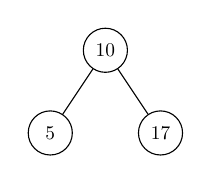
\begin{tikzpicture}[nodeStyle/.style={circle, draw, minimum size=0.8cm}, scale=0.7, transform shape]
                    \node[nodeStyle](root) at (0, 0) {10};
                    \node[nodeStyle](11) at (-1, -1.5) {5};
                    \node[nodeStyle](12) at ( 1, -1.5) {17};

                    \draw (root) -- (11);
                    \draw (root) -- (12);
                \end{tikzpicture}
            \end{center}
        \end{column}
        \begin{column}{0.48\textwidth}
        \end{column}
    \end{columns}
\end{frame}

\begin{frame}[t]
    \frametitle{Aufgabe 9.1 - AVL Bebaumung}
    Insert 1:

    \bigskip
    \bigskip

    \begin{columns}
        \begin{column}{0.48\textwidth}
            \begin{center}
                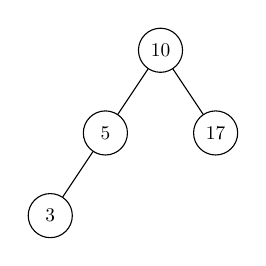
\begin{tikzpicture}[nodeStyle/.style={circle, draw, minimum size=0.8cm}, scale=0.7, transform shape]
                    \node[nodeStyle](root) at (0, 0) {10};
                    \node[nodeStyle](11) at (-1, -1.5) {5};
                    \node[nodeStyle](12) at ( 1, -1.5) {17};
                    \node[nodeStyle](21) at (-2, -3) {3};

                    \draw (root) -- (11);
                    \draw (root) -- (12);
                    \draw (11) -- (21);
                \end{tikzpicture}
            \end{center}
        \end{column}
        \begin{column}{0.48\textwidth}
        \end{column}
    \end{columns}
\end{frame}

\begin{frame}[t]
    \frametitle{Aufgabe 9.1 - AVL Bebaumung}
    Insert 4:

    \bigskip
    \bigskip

    \begin{columns}
        \begin{column}{0.48\textwidth}
            \begin{center}
                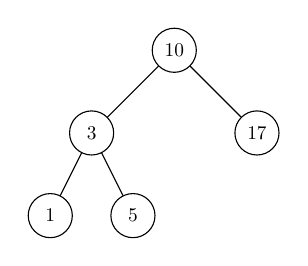
\begin{tikzpicture}[nodeStyle/.style={circle, draw, minimum size=0.8cm}, scale=0.7, transform shape]
                    \node[nodeStyle](root) at (0, 0) {10};
                    \node[nodeStyle](11) at (-1.5, -1.5) {3};
                    \node[nodeStyle](12) at ( 1.5, -1.5) {17};
                    \node[nodeStyle](21) at (-2.25, -3) {1};
                    \node[nodeStyle](22) at (-0.75, -3) {5};

                    \draw (root) -- (11);
                    \draw (root) -- (12);
                    \draw (11) -- (21);
                    \draw (11) -- (22);
                \end{tikzpicture}
            \end{center}
        \end{column}
        \begin{column}{0.48\textwidth}
        \end{column}
    \end{columns}
\end{frame}

\begin{frame}[t]
    \frametitle{Aufgabe 9.1 - AVL Bebaumung}
    Remove 4:

    \bigskip
    \bigskip

    \begin{columns}
        \begin{column}{0.48\textwidth}
            \begin{center}
                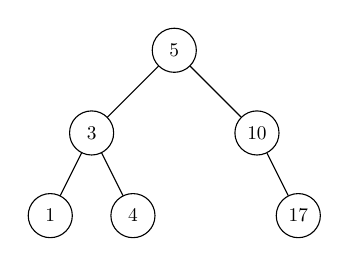
\begin{tikzpicture}[nodeStyle/.style={circle, draw, minimum size=0.8cm}, scale=0.7, transform shape]
                    \node[nodeStyle](root) at (0, 0) {5};
                    \node[nodeStyle](11) at (-1.5, -1.5) {3};
                    \node[nodeStyle](12) at ( 1.5, -1.5) {10};
                    \node[nodeStyle](21) at (-2.25, -3) {1};
                    \node[nodeStyle](22) at (-0.75, -3) {4};
                    \node[nodeStyle](24) at ( 2.25, -3) {17};

                    \draw (root) -- (11);
                    \draw (root) -- (12);
                    \draw (11) -- (21);
                    \draw (11) -- (22);
                    \draw (12) -- (24);
                \end{tikzpicture}
            \end{center}
        \end{column}
        \begin{column}{0.48\textwidth}
        \end{column}
    \end{columns}
\end{frame}

\begin{frame}[t]
    \frametitle{Aufgabe 9.1 - AVL Bebaumung}
    Insert 8:

    \bigskip
    \bigskip

    \begin{columns}
        \begin{column}{0.48\textwidth}
            \begin{center}
                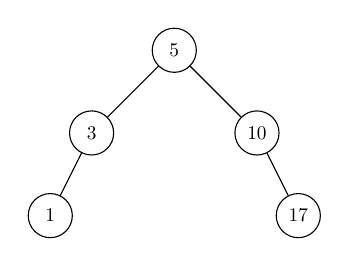
\begin{tikzpicture}[nodeStyle/.style={circle, draw, minimum size=0.8cm}, scale=0.7, transform shape]
                    \node[nodeStyle](root) at (0, 0) {5};
                    \node[nodeStyle](11) at (-1.5, -1.5) {3};
                    \node[nodeStyle](12) at ( 1.5, -1.5) {10};
                    \node[nodeStyle](21) at (-2.25, -3) {1};
                    \node[nodeStyle](24) at ( 2.25, -3) {17};

                    \draw (root) -- (11);
                    \draw (root) -- (12);
                    \draw (11) -- (21);
                    \draw (12) -- (24);
                \end{tikzpicture}
            \end{center}
        \end{column}
        \begin{column}{0.48\textwidth}
        \end{column}
    \end{columns}
\end{frame}

\begin{frame}[t]
    \frametitle{Aufgabe 9.1 - AVL Bebaumung}
    Insert 2:

    \bigskip
    \bigskip

    \begin{columns}
        \begin{column}{0.48\textwidth}
            \begin{center}
                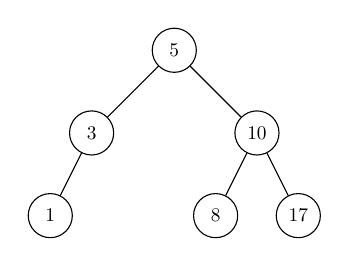
\begin{tikzpicture}[nodeStyle/.style={circle, draw, minimum size=0.8cm}, scale=0.7, transform shape]
                    \node[nodeStyle](root) at (0, 0) {5};
                    \node[nodeStyle](11) at (-1.5, -1.5) {3};
                    \node[nodeStyle](12) at ( 1.5, -1.5) {10};
                    \node[nodeStyle](21) at (-2.25, -3) {1};
                    \node[nodeStyle](23) at ( 0.75, -3) {8};
                    \node[nodeStyle](24) at ( 2.25, -3) {17};

                    \draw (root) -- (11);
                    \draw (root) -- (12);
                    \draw (11) -- (21);
                    \draw (12) -- (23);
                    \draw (12) -- (24);
                \end{tikzpicture}
            \end{center}
        \end{column}
        \begin{column}{0.48\textwidth}
        \end{column}
    \end{columns}
\end{frame}

\begin{frame}[t]
    \frametitle{Aufgabe 9.1 - AVL Bebaumung}
    Insert 7:

    \bigskip
    \bigskip

    \begin{columns}
        \begin{column}{0.48\textwidth}
            \begin{center}
                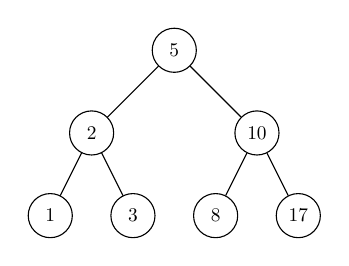
\begin{tikzpicture}[nodeStyle/.style={circle, draw, minimum size=0.8cm}, scale=0.7, transform shape]
                    \node[nodeStyle](root) at (0, 0) {5};
                    \node[nodeStyle](11) at (-1.5, -1.5) {2};
                    \node[nodeStyle](12) at ( 1.5, -1.5) {10};
                    \node[nodeStyle](21) at (-2.25, -3) {1};
                    \node[nodeStyle](22) at (-0.75, -3) {3};
                    \node[nodeStyle](23) at ( 0.75, -3) {8};
                    \node[nodeStyle](24) at ( 2.25, -3) {17};

                    \draw (root) -- (11);
                    \draw (root) -- (12);
                    \draw (11) -- (21);
                    \draw (11) -- (22);
                    \draw (12) -- (23);
                    \draw (12) -- (24);
                \end{tikzpicture}
            \end{center}
        \end{column}
        \begin{column}{0.48\textwidth}
        \end{column}
    \end{columns}
\end{frame}

\begin{frame}[t]
    \frametitle{Aufgabe 9.1 - AVL Bebaumung}
    Insert 6:

    \bigskip
    \bigskip

    \begin{columns}
        \begin{column}{0.48\textwidth}
            \begin{center}
                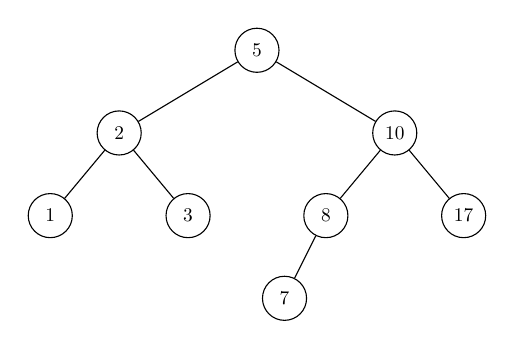
\begin{tikzpicture}[nodeStyle/.style={circle, draw, minimum size=0.8cm}, scale=0.7, transform shape]
                    \node[nodeStyle](root) at (0, 0) {5};
                    \node[nodeStyle](11) at (-2.5, -1.5) {2};
                    \node[nodeStyle](12) at ( 2.5, -1.5) {10};
                    \node[nodeStyle](21) at (-3.75, -3) {1};
                    \node[nodeStyle](22) at (-1.25, -3) {3};
                    \node[nodeStyle](23) at ( 1.25, -3) {8};
                    \node[nodeStyle](24) at ( 3.75, -3) {17};
                    \node[nodeStyle](35) at ( 0.5, -4.5) {7};

                    \draw (root) -- (11);
                    \draw (root) -- (12);
                    \draw (11) -- (21);
                    \draw (11) -- (22);
                    \draw (12) -- (23);
                    \draw (12) -- (24);
                    \draw (23) -- (35);
                \end{tikzpicture}
            \end{center}
        \end{column}
        \begin{column}{0.48\textwidth}
        \end{column}
    \end{columns}
\end{frame}

\begin{frame}[t]
    \frametitle{Aufgabe 9.1 - AVL Bebaumung}
    Insert 9:

    \bigskip
    \bigskip

    \begin{columns}
        \begin{column}{0.48\textwidth}
            \begin{center}
                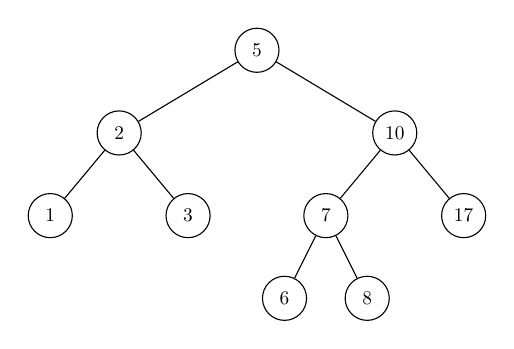
\begin{tikzpicture}[nodeStyle/.style={circle, draw, minimum size=0.8cm}, scale=0.7, transform shape]
                    \node[nodeStyle](root) at (0, 0) {5};
                    \node[nodeStyle](11) at (-2.5, -1.5) {2};
                    \node[nodeStyle](12) at ( 2.5, -1.5) {10};
                    \node[nodeStyle](21) at (-3.75, -3) {1};
                    \node[nodeStyle](22) at (-1.25, -3) {3};
                    \node[nodeStyle](23) at ( 1.25, -3) {7};
                    \node[nodeStyle](24) at ( 3.75, -3) {17};
                    \node[nodeStyle](35) at ( 0.5, -4.5) {6};
                    \node[nodeStyle](36) at ( 2, -4.5) {8};

                    \draw (root) -- (11);
                    \draw (root) -- (12);
                    \draw (11) -- (21);
                    \draw (11) -- (22);
                    \draw (12) -- (23);
                    \draw (12) -- (24);
                    \draw (23) -- (35);
                    \draw (23) -- (36);
                \end{tikzpicture}
            \end{center}
        \end{column}
        \begin{column}{0.48\textwidth}
        \end{column}
    \end{columns}
\end{frame}

\begin{frame}[t]
    \frametitle{Aufgabe 9.1 - AVL Bebaumung}
    Remove 2:

    \bigskip
    \bigskip

    \begin{columns}
        \begin{column}{0.48\textwidth}
            \begin{center}
                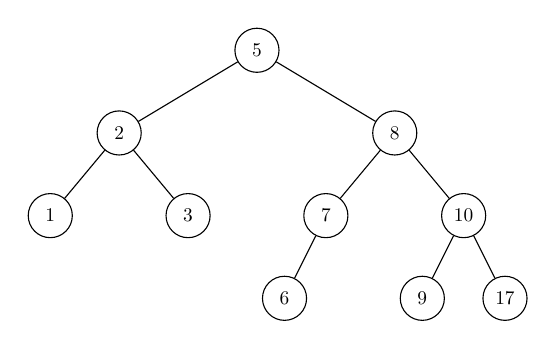
\begin{tikzpicture}[nodeStyle/.style={circle, draw, minimum size=0.8cm}, scale=0.7, transform shape]
                    \node[nodeStyle](root) at (0, 0) {5};
                    \node[nodeStyle](11) at (-2.5, -1.5) {2};
                    \node[nodeStyle](12) at ( 2.5, -1.5) {8};
                    \node[nodeStyle](21) at (-3.75, -3) {1};
                    \node[nodeStyle](22) at (-1.25, -3) {3};
                    \node[nodeStyle](23) at ( 1.25, -3) {7};
                    \node[nodeStyle](24) at ( 3.75, -3) {10};
                    \node[nodeStyle](35) at ( 0.5, -4.5) {6};
                    \node[nodeStyle](37) at ( 3, -4.5) {9};
                    \node[nodeStyle](38) at ( 4.5, -4.5) {17};

                    \draw (root) -- (11);
                    \draw (root) -- (12);
                    \draw (11) -- (21);
                    \draw (11) -- (22);
                    \draw (12) -- (23);
                    \draw (12) -- (24);
                    \draw (23) -- (35);
                    \draw (24) -- (37);
                    \draw (24) -- (38);
                \end{tikzpicture}
            \end{center}
        \end{column}
        \begin{column}{0.48\textwidth}
        \end{column}
    \end{columns}
\end{frame}

\begin{frame}[t]
    \frametitle{Aufgabe 9.1 - AVL Bebaumung}
    Remove 1:

    \bigskip
    \bigskip

    \begin{columns}
        \begin{column}{0.48\textwidth}
            \begin{center}
                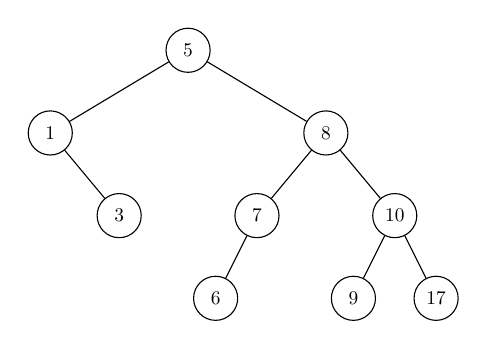
\begin{tikzpicture}[nodeStyle/.style={circle, draw, minimum size=0.8cm}, scale=0.7, transform shape]
                    \node[nodeStyle](root) at (0, 0) {5};
                    \node[nodeStyle](11) at (-2.5, -1.5) {1};
                    \node[nodeStyle](12) at ( 2.5, -1.5) {8};
                    \node[nodeStyle](22) at (-1.25, -3) {3};
                    \node[nodeStyle](23) at ( 1.25, -3) {7};
                    \node[nodeStyle](24) at ( 3.75, -3) {10};
                    \node[nodeStyle](35) at ( 0.5, -4.5) {6};
                    \node[nodeStyle](37) at ( 3, -4.5) {9};
                    \node[nodeStyle](38) at ( 4.5, -4.5) {17};

                    \draw (root) -- (11);
                    \draw (root) -- (12);
                    \draw (11) -- (22);
                    \draw (12) -- (23);
                    \draw (12) -- (24);
                    \draw (23) -- (35);
                    \draw (24) -- (37);
                    \draw (24) -- (38);
                \end{tikzpicture}
            \end{center}
        \end{column}
        \begin{column}{0.48\textwidth}
        \end{column}
    \end{columns}
\end{frame}

\begin{frame}[t]
    \frametitle{Aufgabe 9.1 - AVL Bebaumung}
    Remove 8:

    \bigskip
    \bigskip

    \begin{columns}
        \begin{column}{0.48\textwidth}
            \begin{center}
                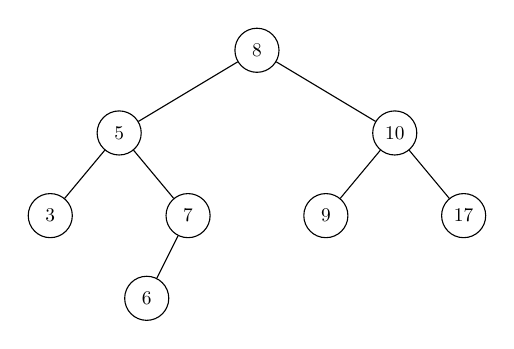
\begin{tikzpicture}[nodeStyle/.style={circle, draw, minimum size=0.8cm}, scale=0.7, transform shape]
                    \node[nodeStyle](root) at (0, 0) {8};
                    \node[nodeStyle](11) at (-2.5, -1.5) {5};
                    \node[nodeStyle](12) at ( 2.5, -1.5) {10};
                    \node[nodeStyle](21) at (-3.75, -3) {3};
                    \node[nodeStyle](22) at (-1.25, -3) {7};
                    \node[nodeStyle](23) at ( 1.25, -3) {9};
                    \node[nodeStyle](24) at ( 3.75, -3) {17};
                    \node[nodeStyle](33) at (-2, -4.5) {6};

                    \draw (root) -- (11);
                    \draw (root) -- (12);
                    \draw (11) -- (21);
                    \draw (11) -- (22);
                    \draw (12) -- (23);
                    \draw (12) -- (24);
                    \draw (22) -- (33);
                \end{tikzpicture}
            \end{center}
        \end{column}
        \begin{column}{0.48\textwidth}
        \end{column}
    \end{columns}
\end{frame}

\begin{frame}
    \frametitle{Aufgabe 9.1 - AVL Bebaumung (Extra Platz)}
\end{frame}